\clearpage

\section{软件构建关键技术}
\label{sec:skills}

本章主要讨论基于Cartesian坐标系和Frenet标架的两种重建算法,
并提出一种改良算法,兼具重建精度高和运行速度快的优点。

另外,本章将讨论渲染引擎、网络传输技术和编程语言的选择。

\subsection{曲线重建算法}
\label{sec:reconst}
曲线重建主要分为两个部分,一个是连续化,即将离散的数据连续化;
另一部分是拟合,根据数据拟合得到绝对坐标系下的曲线各点坐标。
根据传感器的种类不同,所测得的数据类型不同,这两步工作的执行顺序也可以不同。

如MEMS惯性传感器主要测量加速度数据,并对加速度数据进行二次积分而得到测量点位移,
故可以在计算测量点坐标之后再进行连续化;而像FBG传感器所得到的是测量点的曲率数据,
难以直接计算获得该点坐标,必须先对曲率数据进行连续化,然后通过拟合算法计算得出各点的坐标。

本小节主要讨论连续化算法和基于曲率数据的曲线拟合算法。

\subsubsection{连续化算法}
常用的连续化算法有线性插值法、
贝塞尔(Bezier)曲线插值法、
B样条曲线插值法和三次样条曲线插值法。

\begin{enumerate}[label=(\Alph*)]
    \item \textbf{线性插值法} \\
    线性插值法即认为每两个测量点处的曲率变化是线性的,即:
    \begin{equation}
    \left\{
        \begin{array}{lr}
        k_{i, i+1} (S) = a_i (S - S_i) + k_i, \ S_i\leq S\leq S_{i+1}\\
    \\
        a_i = \frac{k_{i+1} - k_i}{S_{i+1} - S_i}
    \\
        k_0 = S_0 = 0
        \end{array}
    \right.
    \end{equation}

    其中$S$为自变量,表示距离原点的曲线弧长,$S_i$为第$i$个测量距原点的弧长;
    $k_i$表示第$i$个测量点的曲率;
    $a_i$表示第$i$个拟合参数;
    $k_{i, i+1}$表示第$i$个测量点到第$i+1$个测量点连线的曲率函数。
    
    线性插值算法简单,计算速度快;但是分割点连接处不平滑,跟实际产生的曲线可能存在一定的差距。

    \item \textbf{贝塞尔曲线插值法} \\
    贝塞尔曲线的一般式如下:

    \begin{equation}
        k(S) = \Sigma_{i=0}^nC_n ^ i a_i(1-S)^{n - i}S^i
    \end{equation}

    贝塞尔曲线插值结果很光滑,但存在另外的问题:

    \begin{enumerate}[label=(\alph*)]
        \item 确定了测量点数$n+1$,也就决定了所定义的Bezier曲线的阶次$n$,无法降阶,很不灵活。
        \item 当测量阶次$n$较大时,曲线的阶次将比较高。此时,测量点对曲线形状的控制将明显减弱。
        \item Bezier的调和函数$\Sigma_{i=0}^nC_n ^ i (1-S)^{n - i}S^i$的值在开区间$(0,1)$内均不为0。
        因此,所定义的曲线在$(0<S<1)$的区间内的任何一点均要受到全部顶点的影响,
        即改变其中任一个顶点的位置,都将对整条曲线产生影响,因此对曲线进行局部修改是不可能的。
    \end{enumerate}

    \item \textbf{B样条曲线插值法} \\
    为了克服以上提到的在Bezier曲线中存在的问题,
    Gordon、Riesenfeld和Forrest等人拓展了Bezier曲线,用n次B样条基函数替换了伯恩斯坦基函数,
    构造了B样条曲线。B样条曲线除了保持Bezier曲线所具有的优点外,还增加了可以对曲线进行局部修改这一突出的优点。
    除此之外,它还具有对特征多边形更逼近以及多项式阶次较低等优点。因此,B样条曲线在外形设计中得到了更广泛的重视和应用。

    \begin{equation}
    \left\{
        \begin{array}{lr}
        k(S) = \Sigma_{i=0}^n a_i B_{i, deg}(S)
    \\
        B_{i, deg}(S) = \frac{S-S_i}{S_{i+deg} - S_i}B_{i, deg-1}(S) +\frac{S_{i + deg +1}-S}{S_{i + deg +1} - S_i}B_{i+1, deg-1}(S) 
        \end{array}
    \right.
    \end{equation}

    上面就是B样条曲线的方程,其中$B(S)$被称为基础函数表,
    基础函数表本质上是个递归方程,同时也是一个中间参数。
    当前$deg$阶的元素需要通过两个$deg-1$阶的元素获得,
    $deg-1$阶的元素则需要通过$deg-2$阶的元素获得……以此类推,且回退到0阶时有: 

    \begin{equation}
    B_{i, 0} = \left\{
        \begin{array}{lr}
        1, \ S_i \le S \le S_{i+1}
    \\
        0, \ S \textless S_i \ or \ S \textgreater S_{i+1}
        \end{array}
    \right.
    \end{equation}

    B样条曲线克服了Bezier曲线遇到的问题,
    但其在多个离散曲率检测点的曲率数据不全在拟合出的曲率连续化曲线上,
    这会产生一定的拟合误差。我们可以采用三次样条曲线插值法来解决这个问题。

    \item \textbf{三次样条曲线插值法} \\
    假设曲率和弧长的关系为:

    \begin{equation}
        k(S) =  a_i + b_i (S - S_i) + c_i  (S - S_i)^2 + d_i (S - S_i)^3
    \end{equation}

    且曲线在第 i 个分割点满足方程:

    \begin{equation}
    \left\{
        \begin{array}{lr}
        k_i(S_i) = C_i
    \\
        k_i(S_{i+1}) = C_{i+1}
    \\
        k_i'(S_{i+1}) = k_{i+1}'(S_{i+1})
    \\
        k_i''(S_{i+1}) = k_{i+1}''(S_{i+1})
        \end{array}
    \right.
    \end{equation}

    即曲率原函数、一阶和二阶微分均满足连续性关系,这就能保证拟合出的曲率曲线是足够光滑的。

    再将此方程组与下式联立:

    \begin{equation}
    \left\{
        \begin{array}{lr}
        k(0) = 0
    \\
        k(S_n) = 0
        \end{array}
    \right.
    \end{equation}

    则可求得$a_i, b_i, c_i, d_i$四个系数的值,最终可通过曲线上每一个点距原点的弧长计算曲率。
\end{enumerate}

\subsubsection{常用拟合算法}
\FloatBarrier
常用的拟合算法有基于Cartesian坐标系的拟合算法和基于Frenet标架的拟合算法。
基于Cartesian坐标系的拟合算法原理如图\ref{fig:cartesian}。

\begin{figure}[b!]
\centering
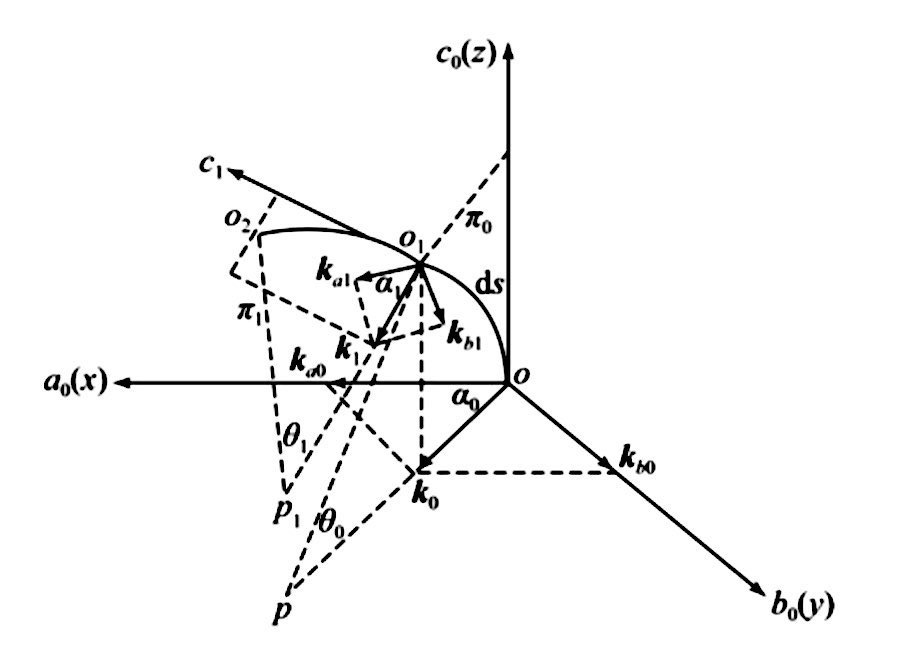
\includegraphics[scale=0.5]{cartesian-coordinate-system.jpg}
\caption{基于Cartesian坐标系的拟合算法\cite{用于光纤光栅曲线重建算法的坐标点拟合}}
\label{fig:cartesian}
\end{figure}

此算法的原理是以每个微段的方向为z轴建立运动坐标系$o_i-a_ib_ic_i$,
并通过几何方法求得下一个点在此坐标系下的相对坐标\cite{3d-shape-display}$o_{i+1} \{d_{ai}, d_{bi}, d_{ci}\}$,
再通过线性变换得到下一个点的运动坐标系\cite{three-dimensional-curve}$o_{i+1}-a_{i+1}b_{i+1} c_{i+1}$。
就可以求得每个点在上个运动坐标系下的相对坐标以及当前坐标系相对上个坐标系的变换矩阵$t_{i, i+1}$。

\FloatBarrier

\begin{align}
    k_i &= \sqrt{k_{ai} ^ 2 + k_{bi} ^ 2}, \\
    \theta_i &= k_i \cdot d_s, \\
    cos\alpha_i &= k_{ai} / k_i, \\
    sin\alpha_i &= k_{bi} / k_i, \\
    d_a &= \frac{cos\alpha_i \cdot (1 - cos\theta_i)}{k_i} \cdot d_s, \\
    d_b &= \frac{sin\alpha_i \cdot (1 - cos\theta_i)}{k_i} \cdot d_s, \\
    d_c &= \frac{sin\theta_i}{k_i} \cdot d_s, \\
    t_{i, i+1} &= \left[
        \begin{matrix}
            cos \alpha_i & -sin \alpha_i & 0 \\
            sin \alpha_i & cos \alpha_i & 0 \\
            0 & 0 & 1
        \end{matrix}
        \right]
        \cdot
        \left[
        \begin{matrix}
            cos \theta_i & 0 & sin \theta_i \\
            0 & 1 & 0 \\
            -sin \theta_i & 0 & cos \theta_i \\
        \end{matrix}
        \right]
        \cdot
        \left[
        \begin{matrix}
            cos \alpha_i & sin \alpha_i & 0 \\
            -sin \alpha_i & cos \alpha_i & 0 \\
            0 & 0 & 1
        \end{matrix}
        \right] \label{alg:reconstruction}
\end{align}

当前坐标系点乘三个矩阵的几何意义分别为:\\
\begin{enumerate}
    \item 绕$\vec c_i$旋转一个$\alpha_i$角使得$\vec a_i$与$\vec k_i$同向;
    \item 绕$\vec b_i$旋转一个$\theta_i$角得到$\vec c_{i+1}$;
    \item 绕$\vec c_{i+1}$旋转一个$-\alpha_i$角得到$\vec a_{i+1}$和$\vec b_{i+1}$。
\end{enumerate}

将变换矩阵累乘即可得到各运动坐标系相对绝对(原点)坐标系的变换矩阵 $T_i$。
然后将相对坐标$o_{i+1} \{d_{ai}, d_{bi}, d_{ci}\}$乘以$T_i$的逆矩阵即可得绝对坐标。

我们也可以使用微分几何中常用的Frenet坐标标架\cite{用于光纤光栅曲线重建算法的坐标点拟合}。令$\vec T$为切向量,$\vec N$为主法向量,指向微段方向;$\vec B$为副法向量,
则有:$\vec B = \vec T \times \vec N$。

假设第$i$段曲线在$xoz$平面内,则两端点平移量$p_{i+1}$有:
\begin{equation}
    p_{i+1} = [-(1-cos \ \theta_i)/k_i \quad 0 \quad sin \ \theta_i/k_i]^T
\end{equation}
曲率$k_i$、弧长$d_s$和弧角$\theta_i$满足$\theta_i = d_s \cdot k_i$。坐标系平移后沿$B_i$轴旋转$\theta_i$,则有:
\begin{equation}
[T_{B_i} ^ {\theta_i}] = \left[
    \begin{matrix}
    cos \theta_i & 0 & -sin \theta_i & 0 \\
    0 &1 & 0 & 0 \\
    sin \theta_i & 0 & cos \theta_i & 0 \\
    0 & 0 & 0 & 1 \\
    \end{matrix}
\right]
\end{equation}
接着将坐标系沿$T_i$旋转$\Delta \phi_{i+1}$,其值由下式求出:
\begin{equation}
\Delta \phi_{i+1} = \begin{cases}
    \phi_{i+1} - \phi_i,&(\phi_{i+1} \ge \phi_i) \\
    2\pi + \phi_{i+1} - \phi_i,&(\phi_{i+1} \textless \phi_i)\\
\end{cases}
\end{equation}
则有:
\begin{equation}
[T_{T_i} ^ {\Delta\phi_{i+1}}] = \left[
    \begin{matrix}
    cos \Delta\phi_{i+1} & -sin \Delta\phi_{i+1} & 0 & 0 \\
    sin \Delta\phi_{i+1} & cos \Delta\phi_{i+1} & 0 & 0 \\
    0 & 0 & 1 & 0 \\
    0 & 0 & 0 & 1 \\
    \end{matrix}
\right]
\end{equation}
由此可求得一个微段运动坐标系的变换矩阵:
\begin{equation}
[t_{i+1}] = \left[
    \begin{matrix}
    & [T_{i+1}] & & p_{i+1} \\
    0 & 0 & 0 & 1 \\
    \end{matrix}
\right]
\end{equation}
其中$[T_{i+1}] = [T_{B_i} ^ {\theta_i}] \cdot [T_{T_i} ^ {\Delta\phi_{i+1}}]$。

通过此变换矩阵即可求得每个点的运动坐标系和下个点的相对坐标,再通过变换矩阵的逆矩阵求得绝对坐标\cite{FBG-sensor-devices},最终拟合出曲线。

\subsubsection{改良拟合算法}

在介绍改良算法之前,先简要介绍Cartesian坐标系二维情况下的曲线重建算法。

\FloatBarrier
\begin{figure}
\centering
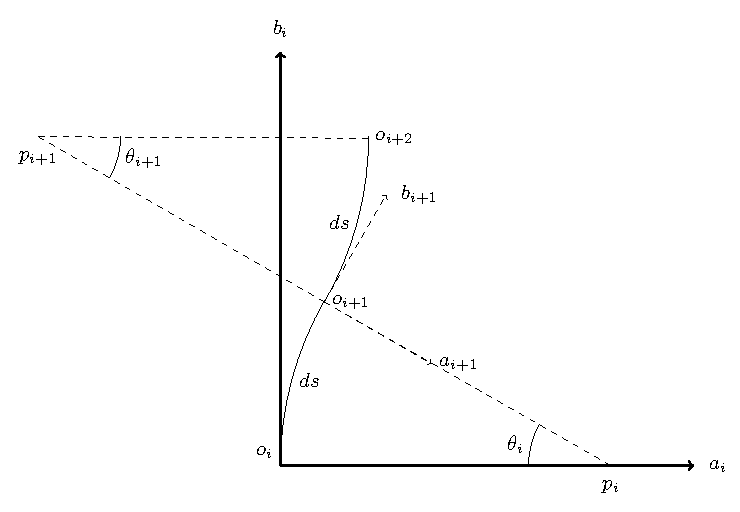
\includegraphics{2d-reconst.pdf}
\caption{基于Cartesian坐标系的二维曲线重建原理}
\label{fig:2d-reconst} 
\end{figure}
\FloatBarrier

如图~\ref{fig:2d-reconst}所示,以曲线的每个$ds$微段的端点$o_i$为原点建立运动坐标系 $o_i-a_ib_i$,
其中$\vec b_i$是曲线在$o_i$点的切向量,$\vec a_i$是法向量。

已知微段曲率值为$k_i$,则有:
\begin{equation}
\theta_i = ds\cdot k_i
\end{equation}
根据几何关系易得:

运动坐标系$o_i-a_ib_i$到运动坐标系$o_{i+1}-a_{i+1}b_{i+1}$的旋转矩阵$r_{i, i+1}$满足:
    \begin{equation}
    r_{i, i+1} = \left[
      \begin{matrix}
      cos \theta_i & sin \theta_i\\
      -sin \theta_i & cos \theta_i\\
      \end{matrix}
    \right]
    \end{equation}
    
$o_{i+1}$在运动坐标系$o_i-a_ib_i$中的相对坐标$t_{i+1}$满足:
    \begin{equation}
    t_{i+1} = \frac{1}{k_i} \cdot \left[
      \begin{matrix}
    	1 - cos\theta_i\\
      sin\theta_i\\
      \end{matrix}
    \right]
    \end{equation}
    
绝对坐标系$o_0-a_0b_0$到运动坐标系$o_i-a_ib_i$的旋转矩阵$R_i$满足:
    \begin{equation}
    R_i = \prod_{k = 0}^{i-1} r_{k, k+1}
    \end{equation}

$o_i$ 到$o_{i+1}$在绝对坐标系中的位移向量$\vec{t_{i+1}}$满足
    \begin{equation}
    \vec{t_{i+1}} = Ri^{-1}\cdot t_{i+1}
    \end{equation}
    
$o_i$在绝对坐标系中的坐标 $T_i$满足:
    \begin{equation}
    T_i = \left[
    		\begin{matrix}
        0\\
        0\\
      	\end{matrix}
      \right]
      + \Sigma_{k=1} ^ {i} \vec{t_i}
    \end{equation}
    
至此,我们通过二维曲线上各微段弧长和曲率拟合出了各端点的绝对坐标。

三维情况下的算法原理如图 ~\ref{fig:coordinate-reconst} 所示,在三维情况下,我们以曲线的每个$ds$微段的端点$o_i$为原点建立运动坐标系\cite{three-dimensional-curve} $o_i-a_ib_ic_i$,
其中$\vec{c_i}$是曲线在$o_i$点的切向量,$\vec{a_i}$是法向量,$\vec{b_i}$是副法向量,则有:
\begin{equation}
\vec{b_i} = \vec{a_i} \times \vec{c_i}
\end{equation}

\FloatBarrier
\begin{figure}[!hbtp]
\centering
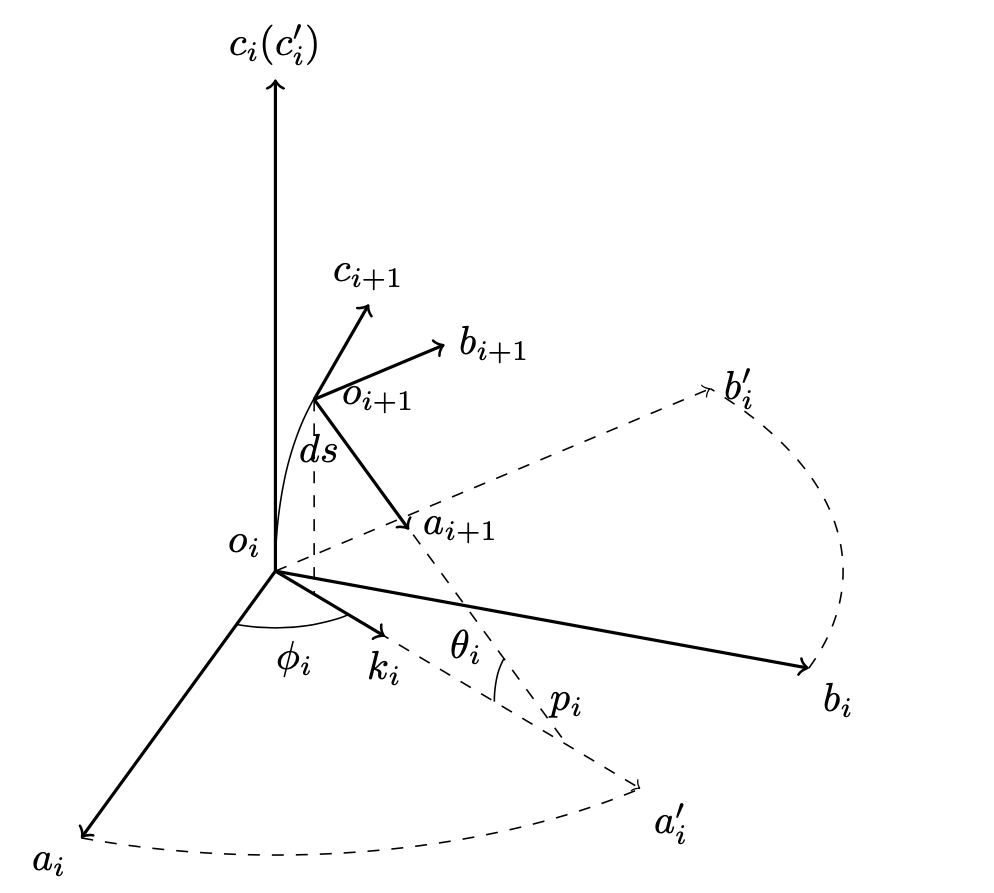
\includegraphics[scale=0.3]{coordinate-reconst.png}
\caption{基于Cartesian坐标系的三维曲线重建原理}
\label{fig:coordinate-reconst} 
\end{figure}

这一点区别于传统的基于Cartesian坐标系的三维曲线重建,运动坐标系不再使用$o_i-x_iy_iz_i$。
这样每次迭代能省去一次矩阵运算,并且可以分别迭代分离旋转矩阵和平移拉伸矩阵。

假设微段合曲率向量为$\vec{k_i}$,则同样有:
\begin{equation}
\theta_i = ds\cdot |\vec{k_i}|
\end{equation}
要求运动坐标系$o_i-a_ib_ic_i$到运动坐标系$o_{i+1}-a_{i+1}b_{i+1}c_{i+1}$的旋转矩阵$r_{i, i+1}$,需先求$\vec{k_i}$与$\vec{a_i}$的夹角$\phi_i$。

已知两个曲率分量$kx$和$ky$,将各运动坐标轴的$o-ab$平面叠加可得到图\ref{fig:iterate-phi}的$o-xy$平面,其中$x$和$y$分别是两个曲率方向。由于$\vec{a}$是曲线法向量,故$\vec{a_{i+1}}$与$\vec{k_i}$同向,即$\vec{a_{i+1}}$与$\vec{a_{i+2}}$的夹角$\phi_{i+1}$是合曲率向量$\vec{k_i}$与$\vec{k_{i+1}}$的夹角。

\begin{figure}[!hbtp]
\centering
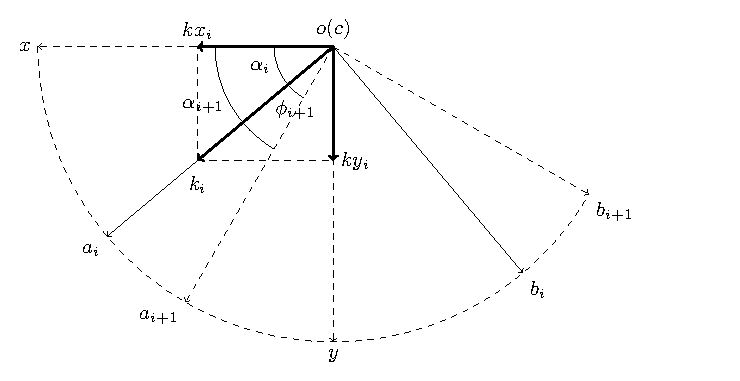
\includegraphics{iterate-phi.pdf}
\caption{运动坐标系旋转俯视图}
\label{fig:iterate-phi} 
\end{figure}

又由于$x$的方向恒定(不发生扭转的情况下),故有:

\begin{align}
\phi_{i+1} &= \alpha_{i+1} - \alpha_i \\
\alpha_i &= arccos\frac{|kx_i|}{|k_i|} \\
k_i &= kx_i + ky_i \\
|k_i| &= \sqrt{(kx_i)^2 + (ky_i)^2}
\end{align}

算得$\phi_i$后可易得:

运动坐标系$o_i-a_ib_ic_i$到临时坐标系$o_i'-a_i'b_i'c_i'$的旋转矩阵$r_i'$满足:
    \begin{equation}
    r_i' = \left[
            \begin{matrix}
            cos\phi_i & -sin\phi_i & 0\\
            sin\phi_i & cos\phi_i & 0\\
            0 & 0 & 1\\
            \end{matrix}
        \right]
    \end{equation}
    
点$o_{i+1}$在临时坐标系$o_i'-a_i'b_i'c_i'$下的相对坐标$o_{i+1}'$满足:
    \begin{equation}
    o_{i+1}' = \frac{1}{|k_i|} \cdot \left[
      \begin{matrix}
    	1 - cos\theta_i\\
    	0 \\
      sin\theta_i\\
      \end{matrix}
    \right]
    \end{equation}
    
临时坐标系$o_i'-a_i'b_i'c_i'$到运动坐标系$o_{i+1}-a_{i+1}b_{i+1}c_{i+1}$的旋转矩阵$r_{i, i+1}$满足:
    \begin{equation}
    r_{i, i+1} = \left[
      \begin{matrix}
      cos \theta_i & 0 & -sin \theta_i\\
      0 &1 & 0\\
      sin \theta_i & 0 & cos \theta_i\\
      \end{matrix}
    \right]
    \end{equation}

绝对坐标系$o_0-a_0b_0c_0$到临时坐标系$o_i'-a_i'b_i'c_i'$的旋转矩阵$R_i'$满足:
    \begin{equation}
    R_i' = r_i' \cdot \prod_{k = 0}^{i-1} r_k' \cdot r_{k, k+1}
    \end{equation}
    
$o_i$ 到$o_{i+1}$在绝对坐标系中的位移向量$\vec{t_{i+1}}$满足:
    \begin{equation}
    \vec{t_i} = Ri'^{-1}\cdot o_{i+1}'
    \end{equation}

绝对坐标原点$o_0$ 到$o_i$的位移向量$\vec{T_i}$满足:
    \begin{equation}
    \vec{T_i} = \Sigma_{k=1} ^ {i} \vec{t_i}
    \end{equation}

即$o_i$在绝对坐标系中的坐标 $T_i$满足\cite{用于光纤光栅曲线重建算法的坐标点拟合}:
\begin{equation}
T_i = \left[
    \begin{matrix}
    0\\
    0\\
    0\\
  	\end{matrix}
  \right]
  + \Sigma_{k=1} ^ {i} \vec{t_i}
\end{equation}
\FloatBarrier

\subsection{渲染引擎选择}
\label{sec:render}

三维渲染是通过电脑计算的方式把模型从三维模型网格呈现出二维真实感高的图像\cite{3DModels_SurveyPaper},
计算过程需要考虑光线及辅助光线、材料的材质和纹理、相机相关设置等综合变量\cite{scientce-of-3d-rendering}。

三维渲染包括实时渲染和非实时渲染。
实时渲染主要应用在游戏领域,电脑会实时的计算和展示所渲染的结果,帧率在20-120左右。
非实时渲染通常是电影或视频,借助计算机有限的算力,通过延长渲染时间达到更加真实的效果。

可视化软件需要实时渲染,本小节主要讨论实时渲染引擎的选择。

常用的实时渲染接口有OpenGL(Open Graphics Library)\cite{opengl}、DirectX(Direct eXtension)\cite{directx}
和Metal\cite{metal}。

OpenGL是一种用于渲染2D或3D图像的跨平台编程接口\cite{opengl},它并不指任何一种特定实现,而是一种接口规范。
DirectX接口仅用于Windows平台,而Metal仅用于Apple平台(macOS、iOS)。为了软件的通用性,本文选择OpenGL作为渲染接口。

OpenGL接口有多个平台的实现,这些平台主要分为原生平台(Native Platform)和浏览器平台(Browser Platform),其中
浏览器平台也称为Web平台。原生平台的软件通常存储在硬盘中并运行在特定操作系统上,
包括C绑定的WGL、GLX和CGL;iOS提供的C绑定和Android提供的Java和C绑定等;
Web平台的软件存储在服务器或浏览器缓存中,运行在浏览器上。
OpenGL的Web平台实现就是JavaScript绑定的WebGL。

WebGL相对于原生渲染引擎有两大优势:
\begin{itemize}
\item 跨平台,操作系统无关,可以在任何大多数浏览器上运行;
\item 易于控制软件版本(热更新、回滚等);
\end{itemize} 

目前支持WebGL的浏览器有:Firefox 4+、Google Chrome 9+、Opera 12+、Safari 5.1+和Internet Explorer 11+
,这些浏览器打开网页即可完成客户端渲染,而无需下载另外的软件或浏览器插件。
同样为了渲染客户端的通用性,本文选择WebGL作为渲染引擎。

Threejs是一个基于WebGL的三维图形库\cite{threejs},它封装了很多实用的图形组件,便于程序构建。

\subsection{网络数据传输技术选择}
\label{sec:net}

既然本文选择了WebGL作为渲染引擎,网络数据传输就必须基于超文本传输协议。

超文本传输协议\cite{rfc7230}(Hyper-Text Transfer Protocol, HTTP)是一个用于传输超媒体文档(例如 HTML)的应用层协议。
它是为Web浏览器与Web服务器之间的通信而设计的。
HTTP遵循经典的客户端-服务端模型,客户端打开一个连接以发出请求,然后等待它收到服务器端响应。
该协议虽然通常基于传输控制协议\cite{rfc793}(Transmission Control Protocol, TCP),但可以在任何可靠的传输层上使用。

HTTP协议目前有1.0,1.1和2.0三个版本,前两个版本是包结构兼容的文本协议;而HTTP/2则是二进制协议\cite{rfc7540},不与HTTP/1.x兼容。

目前使用最广泛的版本是HTTP/1.1。另外,HTTP/1.x协议提供了一种特殊的机制,
这一机制允许将一个已建立的连接升级成新的、不相容的协议。通常来说这一机制总是由客户端发起的
(不过也有例外,比如说可以由服务端发起升级到传输层安全协议\cite{rfc8446}(Transport Layer Security, TLS)),
服务端可以选择是否要升级到新协议。借助这一技术,连接可以以常用的协议启动(如HTTP/1.1),
随后再升级到HTTP/2甚至是WebSocket\cite{rfc6455}。

为了保证软件数据传输的实时性,所使用的传输协议必须支持双向流,以实现原始数据上推客户端到服务器的上推流和服务器到渲染客户端的下推流。
而HTTP/1.x是不支持双向流的,可选的升级方案有WebSocke和gRPC。

WebSocket(简称WS)是浏览器提供的一种浏览器与服务器进行全双工通讯的网络技术,
它是一个独立的协议,但支持使用HTTP/1.x握手。gRPC协议\cite{grpc}是一种由Google制定的远程过程调用(Remote Procedure Call, RPC)协议,
其基于HTTP/2.0和Protocol Buffers\cite{protocol-buffers}。

gRPC性能比WS高,但其Web版本并未得到广泛支持,故本文选择WS作为数据推流协议。

另外,基于TCP的HTTP协议是明文传输且无验证机制的,其存在三大风险:
\begin{enumerate}
    \item 窃听风险(eavesdropping):第三方可以获知通信内容;
    \item 篡改风险(tampering):第三方可以修改通信内容;
    \item 冒充风险(pretending):第三方可以冒充他人身份参与通信(中间人攻击)。
\end{enumerate}

而TLS是为了解决这三大风险而设计的,其设计目标是:

\begin{enumerate}
    \item 所有信息都是加密传播,第三方无法窃听;
    \item 具有校验机制,一旦被篡改,通信双方会立刻发现;
    \item 配备身份证书,防止身份被冒充。
\end{enumerate}

TLS是介于TCP协议和上层应用协议之间的安全层,其作用机理是基于TCP连接建立安全的TLS连接,
再基于TLS连接实现上层协议。
基于TLS的应用层协议都会在原本的协议名后加一个 “S”,如HTTPS、FTPS等,表示此连接是安全的。
为了保证软件的安全性,本文选择基于HTTPS的WSS。

\subsection{编程语言选择}
\label{sec:programming-language}

确定渲染引擎和网络传输协议后,需要选择编程语言以编写软件。
合适的编程语言能同时提升软件开发效率和运行效率。

\subsubsection{Rust}
Rust编程语言\cite{rust}是一门C或C++编程语言的替代语言,它速度与C语言接近且内存利用率极高。
它丰富的类型系统和所有权模型保证了内存安全和线程安全,让开发者在编译期就能够消除内存错误。
另外,它拥有出色的文档、友好的编译器和清晰的错误提示信息,还集成了一流的工具——包管理器和构建工具,
智能地自动补全和类型检验的多编辑器支持,以及自动格式化代码等等。

本文的服务器端程序需要完全承担重建的任务,并需要同时服务多客户端。
为了保证软件的实时性,程序需要高性能和高并发,故适合使用Rust编写。

而数据上推流客户端可能需要运行在ARM等嵌入式平台,计算性能和资源都较为有限,需要较底层的编程语言,
这方面Rust也同样适用。

\subsubsection{TypeScript}
渲染客户端是基于浏览器的,故开发语言必须选择基于JavaScript的编程语言。

TypeScript编程语言\cite{typescript}是一门在JavaScript上构建的静态类型语言。
类型提供了一种描述对象形状的方法,提供了更好的文档,并允许编译器验证代码是否正常工作。
在TypeScript中,标注类型可以是可选的,
编译器强大的类型推断能力可使开发者无需大量标注即可享受代码补全、静态检查等高级开发功能和更舒适的开发体验。

\subsection{本章小结}
本章主要介绍可视化软件构架所需的关键技术。
其中改良的重建算法能准确而快速地根据连续化数据重建出曲线的空间各点坐标;
HTTPS和WebSocket可以将服务端重建的坐标数据安全又实时地传输到客户端渲染程序;
OpenGL和Threejs可以根据曲线各点坐标,跨平台渲染出三维图形;
Rust和TypeScript可以轻松地构建出高性能又易于维护的程序。

然而,这些软件技术的应用需要以实际程序为载体。具体软件的构建细节将在
第\ref{sec:server}章\nameref{sec:server}和第\ref{sec:client}章\nameref{sec:client}中介绍。

\clearpage

\section{服务器端程序实现}
\label{sec:server}
本章主要介绍服务器端程序的实现,主要内容包括数据上推流注册模块、曲线重建模块和数据下推流订阅模块,
并在最后分析算法实现的重建效果与误差。
 
\subsection{数据上推流注册模块}
这个模块需要接收客户端上推的原始数据。所使用的协议为WSS。
本文选用的Web Server是hyper\cite{hyper},并基于它实现了一个简单的Web框架roa\cite{roa}。

hyper是一个专注正确性和高性能的http库,但过于底层,使用不便。
roa是一个类koajs\cite{koajs}的web框架,灵活而易于拓展。
数据上推流注册模块基于roa框架的HTTPS和WebSocket支持,给每个注册的数据源分配唯一的$id$。

数据源注册请求就是一个WebSocket请求:

\begin{lstlisting}[label={lst:register-source},caption={发起数据源注册请求}]
websocket wss://host:port/upstream/
\end{lstlisting}

连接建立之后服务器端给客户端发一个确认包,以告知注册的频道$id$。

\begin{lstlisting}[language=json,firstnumber=1,label={lst:register-resp},caption={数据源注册成功}]
{
    "id": 1
}
\end{lstlisting}

我们采用JSON\cite{rfc7159}作为主要的数据传输序列化格式,这段数据告诉客户端注册频道$id$为$1$,数据上推准备已完成。

其逻辑伪代码如下:

\begin{lstlisting}[caption={注册数据源}]
for connection in incomming() {
    id := sources.push(connection)
    connection.send({"id": id})
}
\end{lstlisting}

其中$incomming$函数接受新的请求连接,$sources$数据源频道列表。
原始数据即传感器直接或间接测得的曲率数据,其内容如代码块 ~\ref{lst:raw-data}中所示。

\subsection{曲线重建模块}
图形学上常用的连续化算法(曲线)有贝塞尔(Bezier)曲线、B样条曲线、Catmull Rom样条曲线等;
而统计学上常用线性插值、多项式插值等。图形学连续化的常见目的是得到光滑曲线,而统计学则追求最小偏差。
由于“曲率光滑程度对曲线重建结果的影响”尚无理论研究,也超出了本文的研究范围,故本文采用其中最简便的线性插值法。

线性插值的实现比较简单,先算出两个方向曲率$k_a$,$k_b$变化的斜率$k_{k_a}$,$k_{k_b}$,
再根据斜率和插值步长$d_s$进行插值。其伪代码如下:

\begin{lstlisting}[caption={线性插值法}]
raw := raws.first()
for next_raw in raws {
    s := next_raw.s - raw.s
    kka := (next_raw.ka - raw.ka) / s
    kkb := (next_raw.kb - raw.kb) / s
    for i in range(0, s / ds) {
        curvatures.push({
            "ka": raw.ka + kka * i, 
            "kb": raw.kb + kkb * i,
        })
    }
    raw = next_raw
}
\end{lstlisting}

其中$raws$为一组原始数据,其每个成员数据都包含一个测量点的弧长曲率数据;
$ds$为采用的插值步长;
$curvatures$为插值后的曲率数据。
得到连续化后的曲率数据 $curvatures$ 如代码块 ~\ref{lst:curvature-vec}中所示。

曲线重建算法需要的运算(如加减乘除、三角函数、平方开方和矩阵运算)Rust语言库均有提供。核心逻辑伪代码如下:

\begin{lstlisting}[caption={曲线重建}]
for ka, kb in curvatures {
    k := sqrt(ka ^ 2 + kb ^ 2)
    theta := k * ds
    alpha := cos(ka / k)
    phi := alpha - alpha_last
    da := (1 - cos(theta)) / k
    db := 0
    dc := sin(theta) / k

    ri = Matrix3::new(
        cos(phi), -sin(phi), 0,
        sin(phi), cos(phi), 0,
        0, 0, 1,
    ) * ri

    ti = (1 / ri) * [da, db, dc]
    ai += ti
    [x, y, z] := ai.column(0)
    points.push(Point {x, y, z})

    ri = Matrix3::new(
        cos(theta), 0, sin(theta),
        0, 1, 0,
        -sin(theta), 0, cos(theta),
    ) * ri
}
\end{lstlisting}

其中$ri$为旋转矩阵,初始值等于单位矩阵;$ti$为每个微元内的平移矩阵;$ai$为总平移矩阵。
重建出的坐标点数据如代码块~\ref{lst:positions}所示。

\subsection{数据下推流订阅模块}

重建数据订阅请求同样是一个WebSocket请求:

\begin{lstlisting}[label={lst:subscribe},caption={重建数据订阅}]
websocket wss://host:port/downstream/:id
\end{lstlisting}

其中的$:id$为频道$id$,在上推数据源注册时获得。
重建数据下推流中的一份数据样例如代码块 ~\ref{lst:positions}所示。
其逻辑伪代码如下:

\begin{lstlisting}[caption={订阅数据源}]
for id, connection in incomming() {
    source := sources.get(id)
    connection.subscribe(source)
}
\end{lstlisting}

\subsection{重建效果与误差分析}
\label{sec:error-analyze}

本节主要内容是重建算法的效果展示与误差分析。
为了便于画图和分析,所用构建对象为二维标准余弦曲线。
在二维标准余弦曲线的第一个周期内,间隔$\frac{\pi}{4}$取采样点以生成原始数据。

本小节中“绝对误差”指在任意$x=x_i$处,标准曲线$y$轴坐标$y_i$与重建曲线$y$轴坐标$y_i'$之差的绝对值;
而“相对误差”指在任意$x=x_i$处,“绝对误差”除以此处标准曲线弧长$s_i$。

\subsubsection{结果与误差}
\FloatBarrier
图~\ref{fig:cos}为插值步长为$0.01$时的余弦曲线重建结果。
其中图~\ref{cos:result}为重建结果对比图,横、纵轴分别为空间中的$x$、$y$坐标;
图~\ref{cos:error}展示了随横坐标$x$变化的绝对误差;
图~\ref{cos:relative-error}展示了随横坐标$x$变化的相对误差。

\begin{figure}
\centering
\subfloat[重建结果]{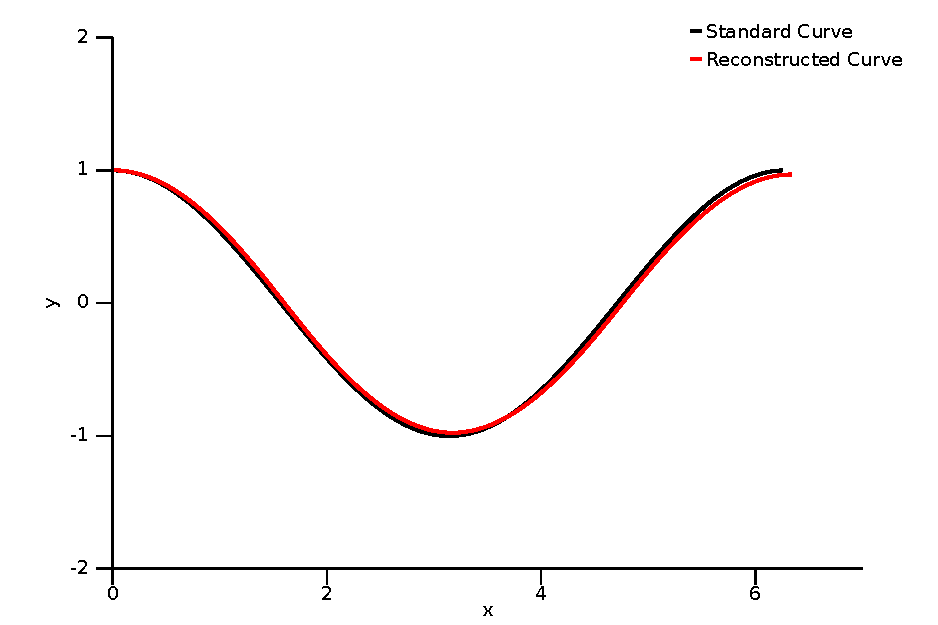
\includegraphics{cos.pdf}\label{cos:result}}\\
\subfloat[绝对误差]{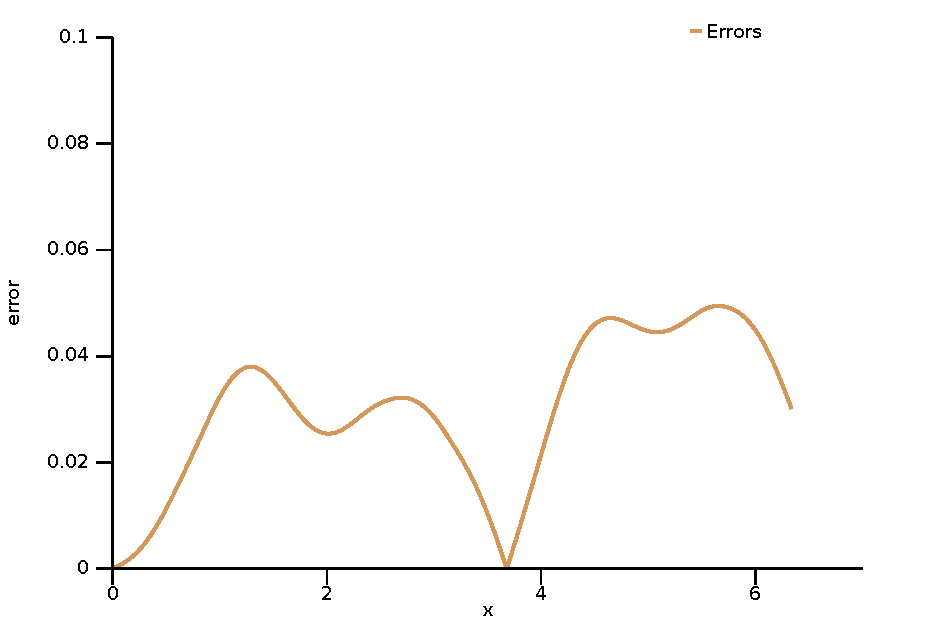
\includegraphics[scale=0.5]{cos-error.pdf}\label{cos:error}}
\subfloat[相对误差]{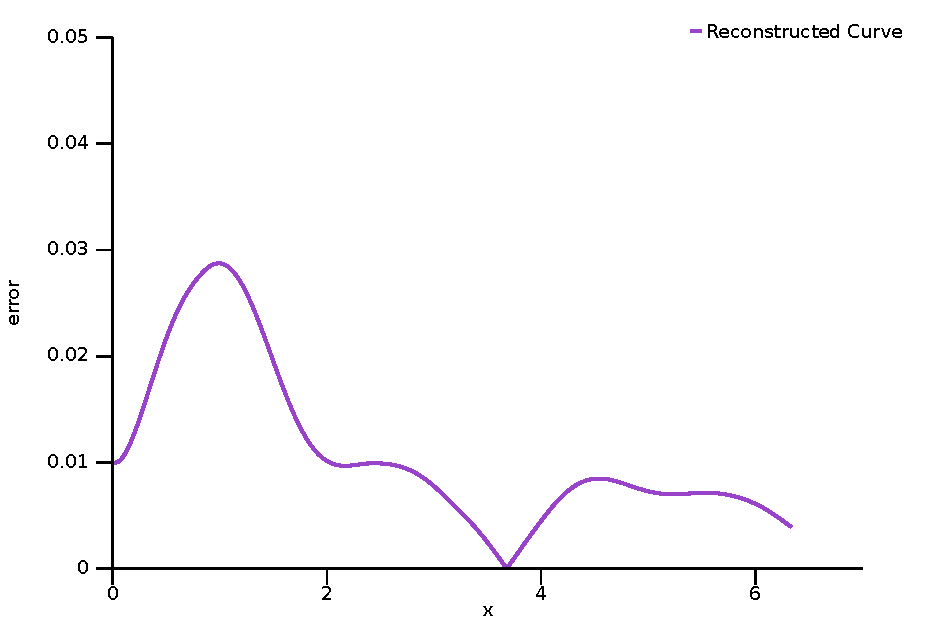
\includegraphics[scale=0.5]{cos-relative-error.pdf}\label{cos:relative-error}}\\
\caption{余弦曲线重建结果与误差}
\label{fig:cos}
\end{figure}

由图可知标准余弦曲线一个周期内的绝对误差在$0.05$以内,而相对误差在$0.03$以内,重建曲线与标准曲线具有高度一致的趋势。

多维曲线重建的过程本质上是一个多元积分,主要误差来自微段内的曲率变化。
当步长$d_s$满足$lim_{d_s\rightarrow 0}$时误差最小。

如果将重建曲线$y$坐标大于标准曲线称为“正误差”,反之则为“负误差”。
那对凹函数曲线而言,误差的增量为正,正误差增大,负误差减小;凸函数则相反。

在标准余弦函数第一个周期内,$x$区间$[0, \frac{\pi}{2})$、$[\frac{3\pi}{2}, 2\pi)$上为凹函数,
在$x$区间$[\frac{\pi}{2}, \frac{3\pi}{2})$上为凸函数,故有:

\begin{itemize}
\item 区间$[0, \frac{\pi}{2})$上误差的增量为正,误差也为正,误差递增;
\item 区间$[\frac{\pi}{2}, \frac{3\pi}{2})$上误差的增量为负;误差为正则减小,减小到零后又增大;
\item 区间$[\frac{3\pi}{2}, 2\pi)$上误差的增量为正;误差为正则增大,误差为负则减小;
\end{itemize}

与重建结果比较可知实际误差变化与理论大致相符。

\FloatBarrier

\subsubsection{不同步长下的误差}
\FloatBarrier

图~\ref{fig:cos-diff-step}为不同插值步长下的余弦曲线重建结果。
其中图~\ref{cos-diff-step:result}为重建结果对比图,横、纵轴分别为空间中的$x$、$y$坐标;
图~\ref{cos-diff-step:error}展示了随横坐标$x$变化的绝对误差;
图~\ref{cos-diff-step:relative-error}展示了随横坐标$x$变化的相对误差。

\begin{figure}
\centering
\subfloat[重建结果]{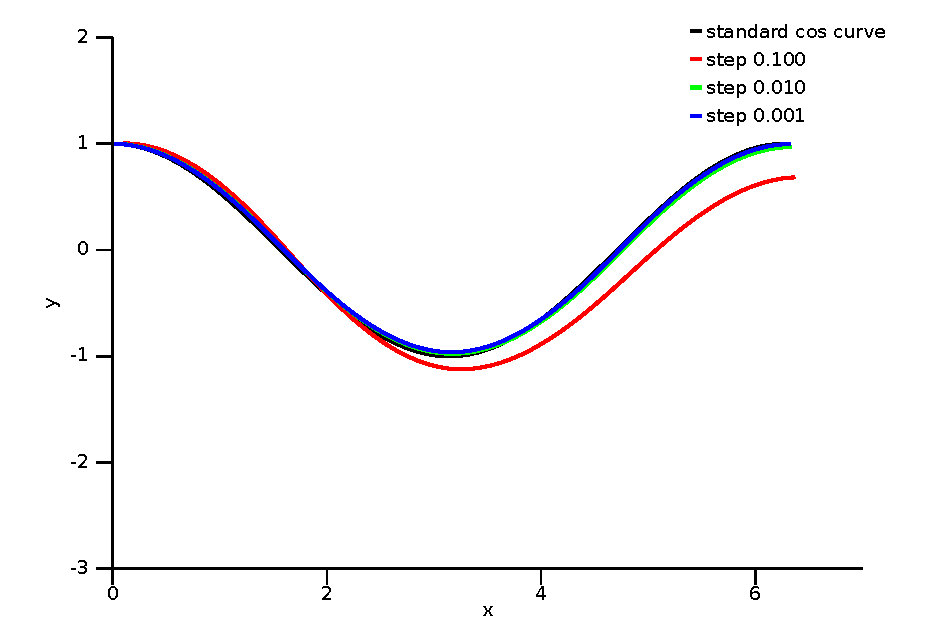
\includegraphics{cos-diff-step.pdf}\label{cos-diff-step:result}}\\
\subfloat[绝对误差]{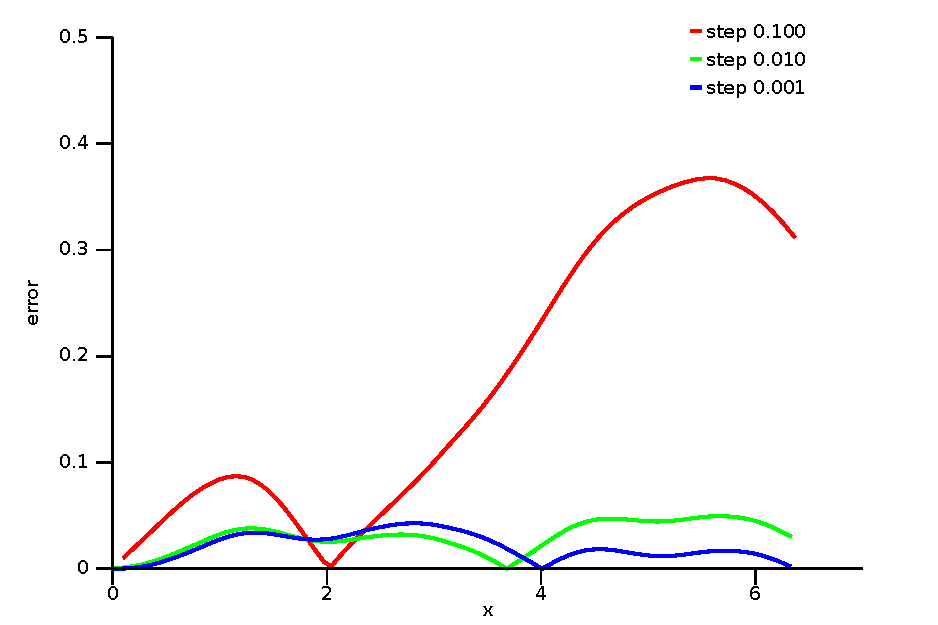
\includegraphics[scale=0.5]{cos-diff-step-error.pdf}\label{cos-diff-step:error}}
\subfloat[相对误差]{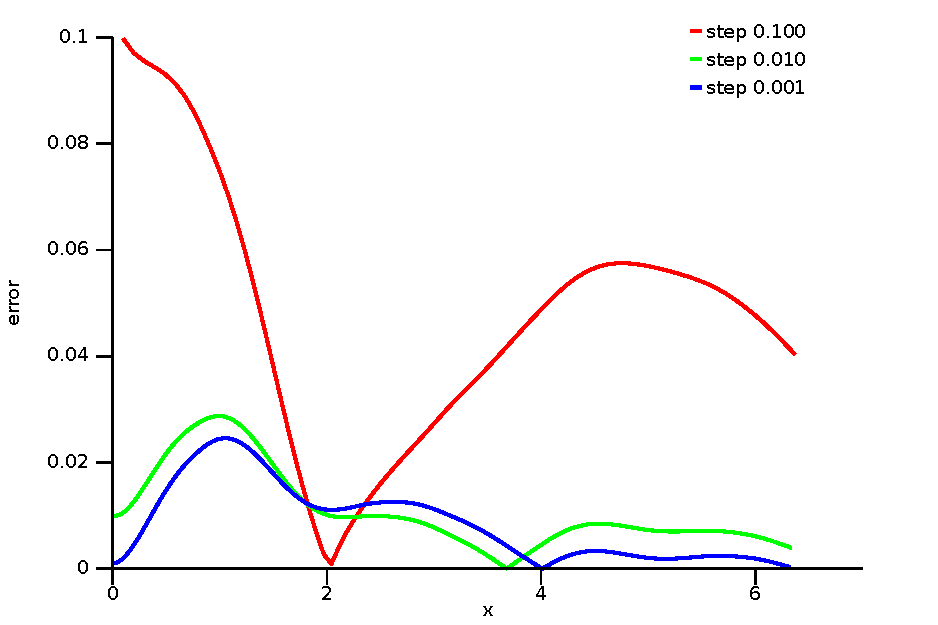
\includegraphics[scale=0.5]{cos-diff-step-relative-error.pdf}\label{cos-diff-step:relative-error}}\\
\caption{不同步长下的余弦曲线重建}
\label{fig:cos-diff-step}
\end{figure}

可见重建误差趋势符合预期,误差增量绝对值与插值步长正相关。
但步长从$0.01$减少到$0.001$带来的准确性提升并不是很明显,却增加了十倍的计算负担,
故$0.01$的插值步长更适于本文软件构建。

\FloatBarrier

\subsection{本章小结}
本章主要介绍服务器端程序的实现细节,并分析了重建结果与误差。
实际误差变化趋势与理论大致相符,可认为算法实现正确;
在$0.01$的插值步长下标准余弦曲线重建的相对误差在$0.03$以内,可以认为重建准确度良好;
另外,在比较了$0.1$、$0.01$、$0.001$三种插值步长下的重建结果后可以认为$0.01$的插值步长更适于本文软件构建。

\clearpage

\section{客户端程序实现}
\label{sec:client}
本章主要介绍两个客户端程序的实现,它们分别是原始数据推流客户端和渲染客户端。

\subsection{原始数据推流客户端}
原始数据推流客户端需要跟传感器对接,直接获得原始曲率数据,对性能的要求不高,但需要支持TCP网络栈。
本文同样使用Rust构建程序,可以运行在ARM架构的计算机上,并可以使用hyper客户端的WebSocket扩展库。

原始数据推流客户端程序核心逻辑如下:

\begin{enumerate}
\item \textbf{注册数据源:}如代码块~\ref{lst:register-source}和~\ref{lst:register-resp}所示;
\item \textbf{上推数据:} \\
伪代码如下:

\begin{lstlisting}[caption={上推数据}]
for raw_data in sense() {
    connection.send(raw_data)
}
\end{lstlisting}

其中$sense$函数会持续地返回原始数据,之后再通过WebSocket连接将数据发往服务器端。

\end{enumerate}

\subsection{渲染客户端}

渲染客户端的主要功能是根据服务器下推的点列实时渲染管壁或轴线。
三维渲染采用WebGL渲染引擎和Threejs库,并使用TypeScript构建。

\subsubsection{数据订阅模块}
渲染流程的第一步是向服务器订阅重建的坐标数据,并根据坐标数据拟合一条Catmull Rom曲线。
数据订阅请求使用浏览器提供的WebSocket接口\cite{mdn-websocket},
曲线拟合使用Threejs提供的$CatmullRomCurve3$。

数据订阅流程如下:

\begin{enumerate}
\item \textbf{订阅数据源:}如代码块~\ref{lst:subscribe}所示;
\item \textbf{接收数据:} \\
重建坐标数据的格式见代码块 ~\ref{lst:positions},逻辑伪代码如下:

\begin{lstlisting}[caption={订阅数据}]
for points in receive() {
    curve := new CatmullRomCurve3(points)
}
\end{lstlisting}

其中$receive$函数会持续地接收坐标数据$points$,之后再基于坐标数据拟合曲线。

\end{enumerate}

\subsubsection{轴线渲染}

获得曲线之后,先考虑渲染一条轴线。
三维渲染的一条线是不需要考虑直径等几何属性的,只需要指定基曲线和基础线材料即可完成渲染。
基础线材料采用Threejs提供的$LineBasicMaterial$,并另外使用其提供的$BufferGeometry$作为动态曲线的缓冲区。
伪代码如下:

\begin{lstlisting}[caption={渲染轴线}]
material := new LineBasicMaterial()
bufGeometry := new THREE.BufferGeometry()
object := new Line(bufGeometry, material)
for points in receive() {
    curve := new CatmullRomCurve3(points)
    bufGeometry.setCurve(curve)
}
\end{lstlisting}

\subsubsection{管壁渲染}

管壁是一个三维物体,它有固定的直径等几何属性和反光度等材料属性,构建过程比轴线更复杂。

本文使用Threejs提供的$MeshPhongMaterial$材质,它是一种光亮的材质,可以模拟具有镜面高光的光泽表面。
渲染一个使用网格材质,双边渲染,分段数$64$,直径$0.1$,反光度$100$的管壁伪代码如下:

\begin{lstlisting}[caption={渲染管壁}]
material := new MeshPhongMaterial({
    shininess: 100,
    side: THREE.DoubleSide,
})
geometry = new TubeGeometry(curve, 64, 0.1)
object := new Mesh(geometry, material)
\end{lstlisting}

\subsubsection{控制器}
控制器是一种响应外部输入(如鼠标键盘)以控制摄像头或其它物体位置、大小、形状的程序模块。
本文主要使用的控制器为轨道控制器,摄像头可以响应鼠标动作绕某一点三轴旋转、缩放,
或是响应键盘上下左右键平移。

轨道控制器使用Threejs提供的$OrbitControls$,其围绕原点旋转伪代码如下:

\begin{lstlisting}[caption={轨道控制器}]
orbitControls := new OrbitControls(camera)
orbitControls.target = [0, 0, 0]
\end{lstlisting}

\subsubsection{环境光}

没有施加环境光照的场景下摄像头是无法成像的。常用的环境光主要有三类:全局光、平行光和点光源。
全局光均匀地照射在场景的每一个物体上,不会产生阴影或者反光,非常易于计算但过于朴素;
平行光会产生阴影和反光效果,并且相对易于计算;点光源计算难度较大,但视觉效果较好。

本文使用一个RGB颜色为\#111111的全局光和一个颜色为\#505050的点光源组成复合光源,
点光源位于空间中坐标$[0, 1000, 0]$处。
全局光和点光源分别使用Threejs提供的$AmbientLight$和$DirectionalLight$,
伪代码如下:

\begin{lstlisting}[caption={环境光}]
scene.add(new AmbientLight(0x111111))
spotLight := new DirectionalLight(0x505050)
spotLight.position.set(0, 1000, 0)
scene.add(spotLight)
\end{lstlisting}

\subsection{本章小结}
本章主要讨论客户端软件的构建。原始数据推流客户端主要负责将传感器感测的数据转为原始数据的格式并上推给服务器;
渲染客户端主要负责接收服务器下推的坐标数据并渲染出三维图形,以及给终端用户提供必要的交互功能。

至此软件的构建已介绍完毕,下一章将展示软件的实际运行效果。

\clearpage

\section{软件运行展示}
\label{sec:pre}
本章将介绍客户端与服务器端对接后,软件整体的使用说明和渲染效果。
展示所用曲线为$[0, 2\pi]$区间内的动态三维余弦曲线,
实时动态展示网址:\\ \href{https://curve.hexilee.me:8000/}{https://curve.hexilee.me:8000/}。

\subsection{使用说明}
\FloatBarrier

图 ~\ref{fig:tube-default} 是软件的默认渲染结果。
界面左上角是帧率监控,如图 ~\ref{fig:fps} 表示帧率区间$18-60$,当前帧率$60$。
界面顶端为交互说明:

\begin{itemize}
\item 鼠标拖拽:旋转视角
\item 滚轮滚动:旋转视角
\item 上下左右键:平移视角
\end{itemize}

界面右上角为控制面板,用于控制渲染选项。
如图 ~\ref{fig:control-pad} 为默认选项,各选项的可选值和含义分别为:

\begin{enumerate}
\item \textbf{mode: }渲染模式,可选择管壁渲染或者轴线渲染;
\item \textbf{color: }轴线或管壁的颜色,手动填入十六进制RGB值;
\item \textbf{backgroundColor: }背景颜色,手动填入十六进制RGB值;
\item \textbf{axes: }勾选显示坐标轴;
\item \textbf{grid: }勾选显示辅助栅格;
\end{enumerate}

\begin{figure}
\centering
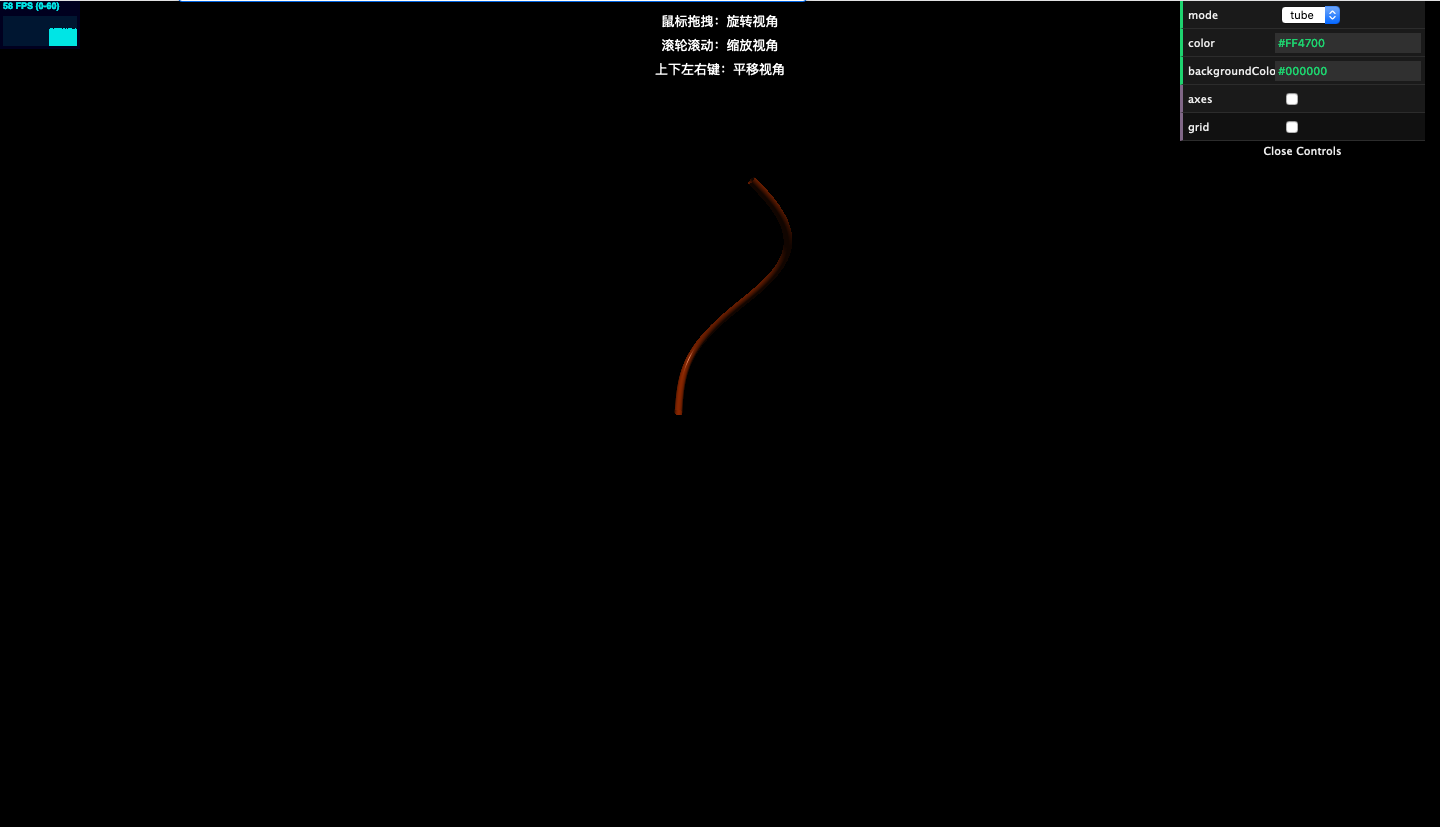
\includegraphics[scale=0.3]{tube-default.png}
\caption{管壁渲染}
\label{fig:tube-default}
\end{figure}

\begin{figure}
\centering
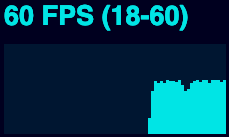
\includegraphics[scale=0.3]{fps.png}
\caption{帧率监控}
\label{fig:fps}
\end{figure}

\begin{figure}
\centering
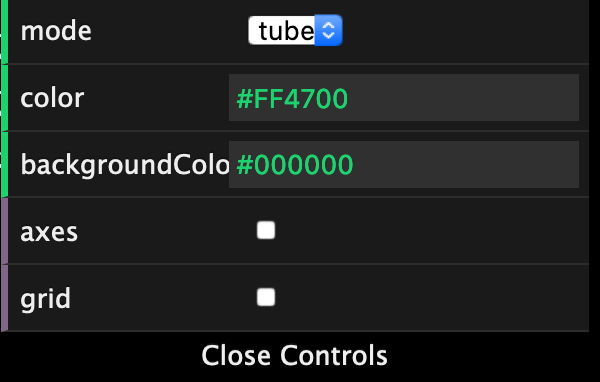
\includegraphics[scale=0.3]{control-pad.png}
\caption{控制面板}
\label{fig:control-pad}
\end{figure}
\FloatBarrier

\subsection{渲染效果}
上一节中展示了默认的渲染效果并介绍了软件界面和使用说明,
本节将会展示在各种选项下的渲染效果。

\begin{enumerate}

\item \textbf{改变管壁颜色} \\
改变管壁颜色为\#00FFFF:
\begin{figure}[H]
\centering
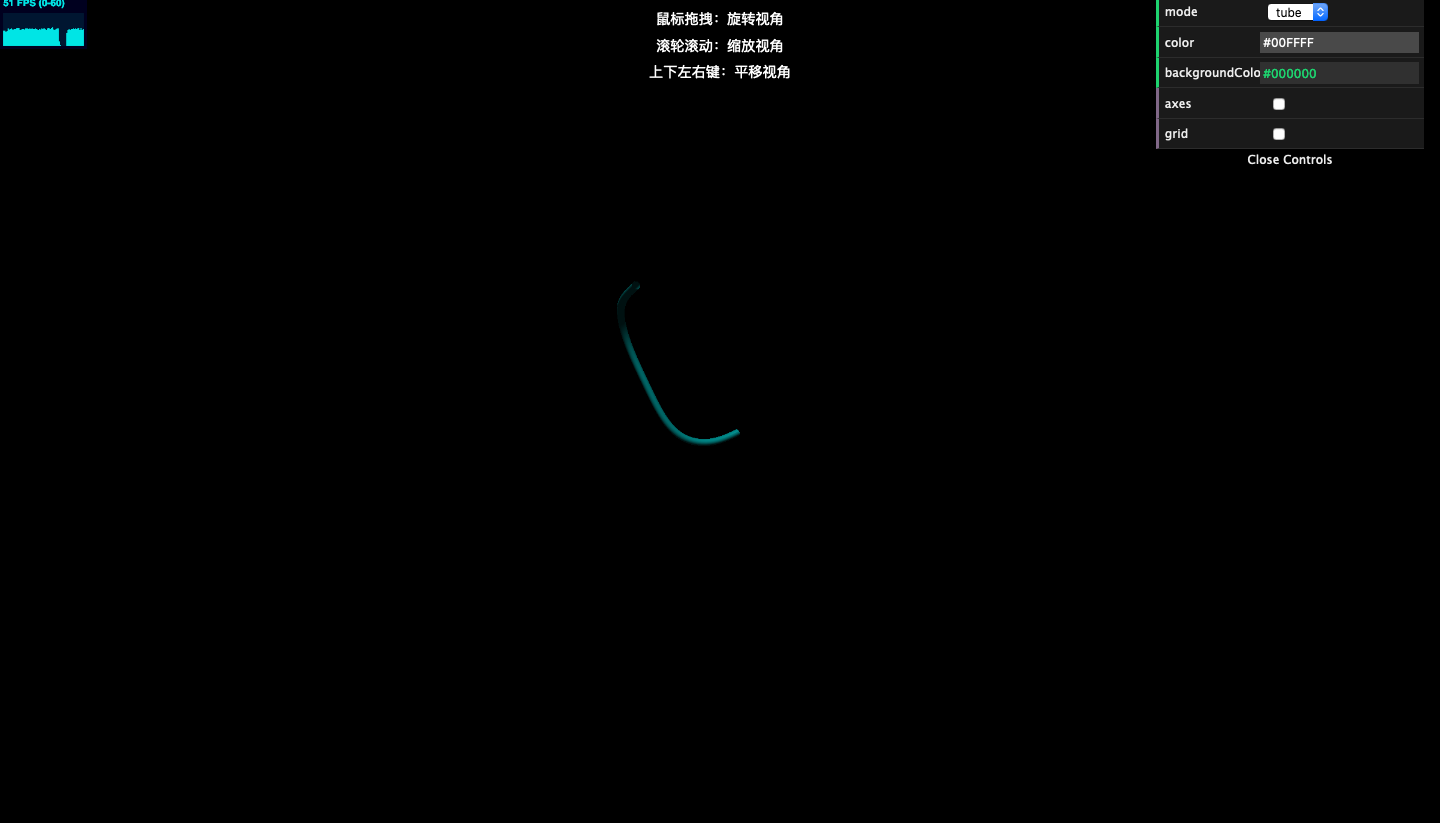
\includegraphics[scale=0.3]{change-color.png}
\caption{改变管壁颜色}
\label{fig:change-color}
\end{figure}

\item \textbf{改变背景颜色} \\
改变背景颜色为\#222222:

\begin{figure}[H]
\centering
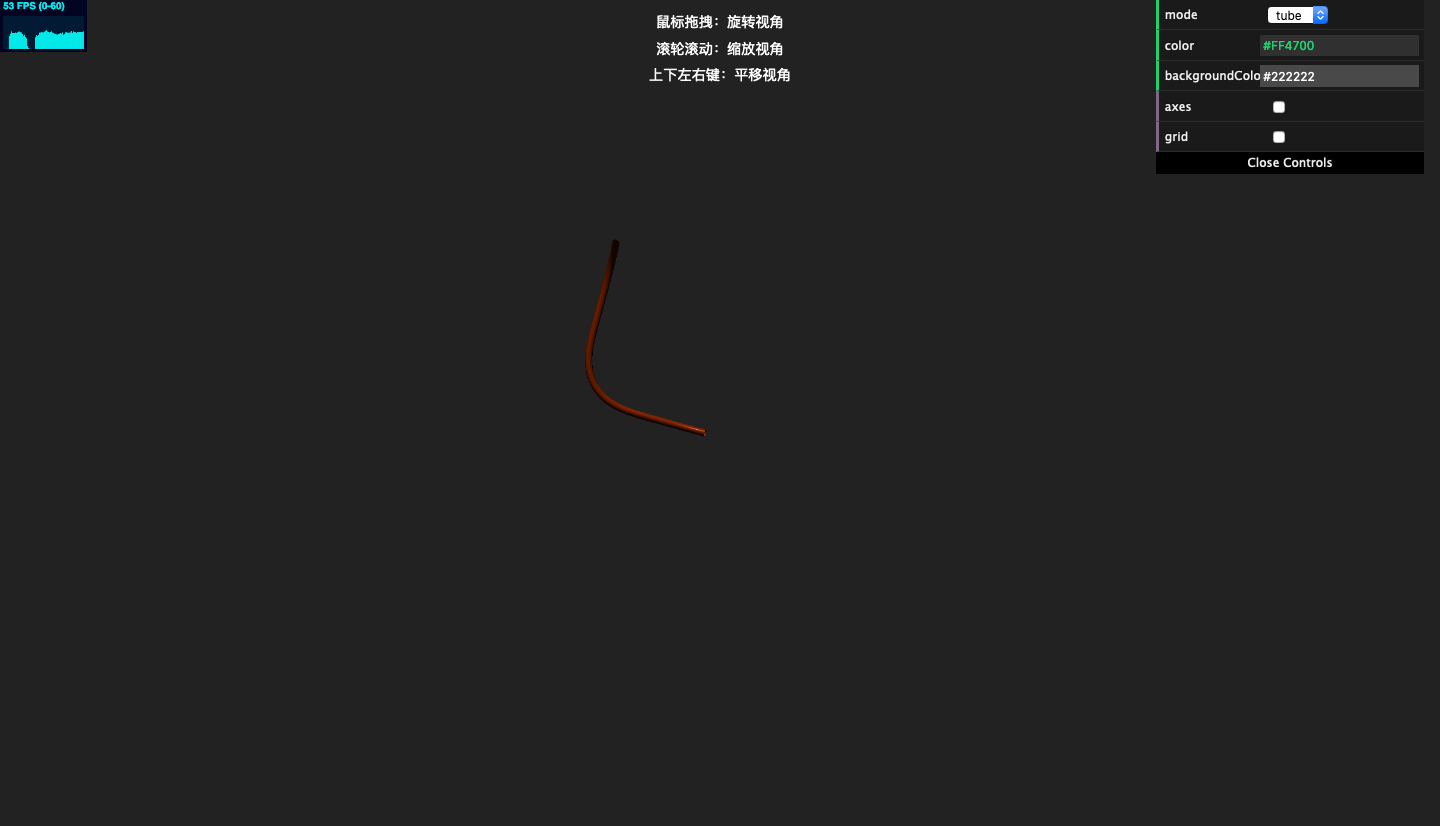
\includegraphics[scale=0.3]{change-bg-color.png}
\caption{改变背景颜色}
\label{fig:change-bg-color}
\end{figure}

\item \textbf{启用坐标轴} \\
勾选选项$axes$:

\begin{figure}[H]
\centering
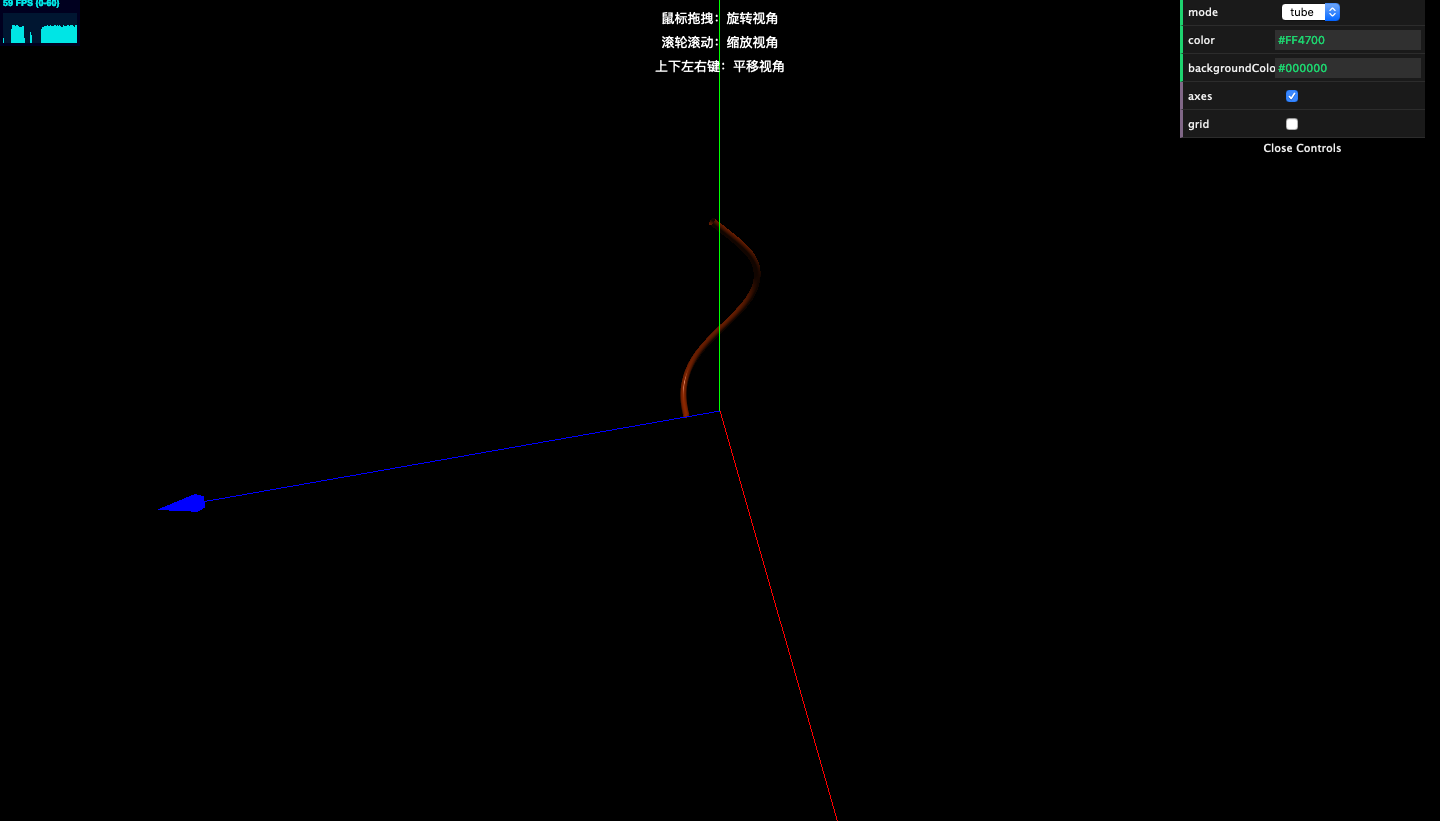
\includegraphics[scale=0.3]{tube-with-axes.png}
\caption{启用坐标轴}
\label{fig:tube-with-axes}
\end{figure}

\item \textbf{启用坐标轴和栅格} \\
勾选选项$axes$和$grid$:

\begin{figure}[H]
\centering
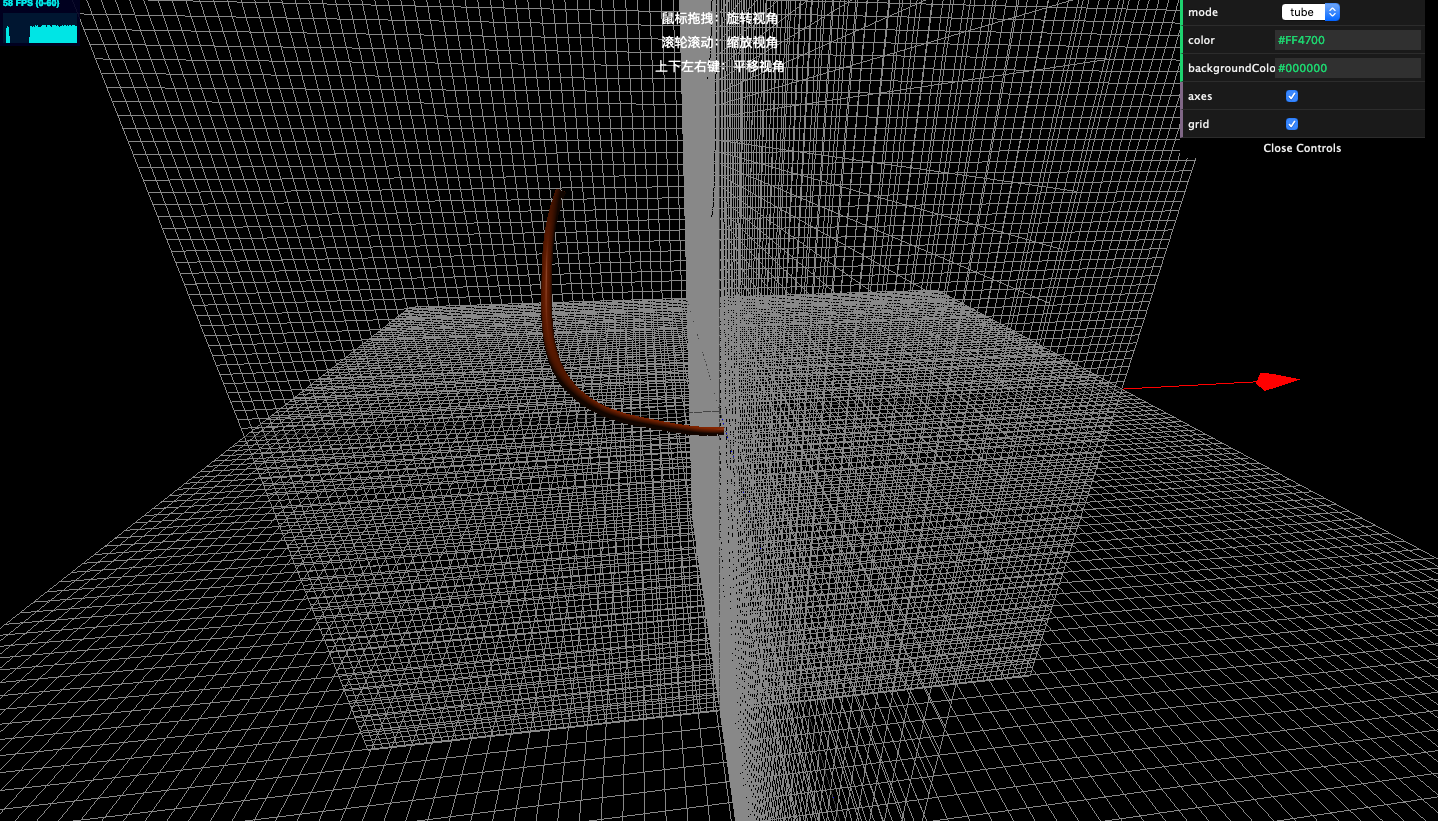
\includegraphics[scale=0.3]{tube-with-axes-grid.png}
\caption{启用坐标轴和栅格}
\label{fig:tube-with-axes-grid}
\end{figure}

\item \textbf{轴线渲染} \\
渲染模式$mode$切换到选项$line$:

\begin{figure}[H]
\centering
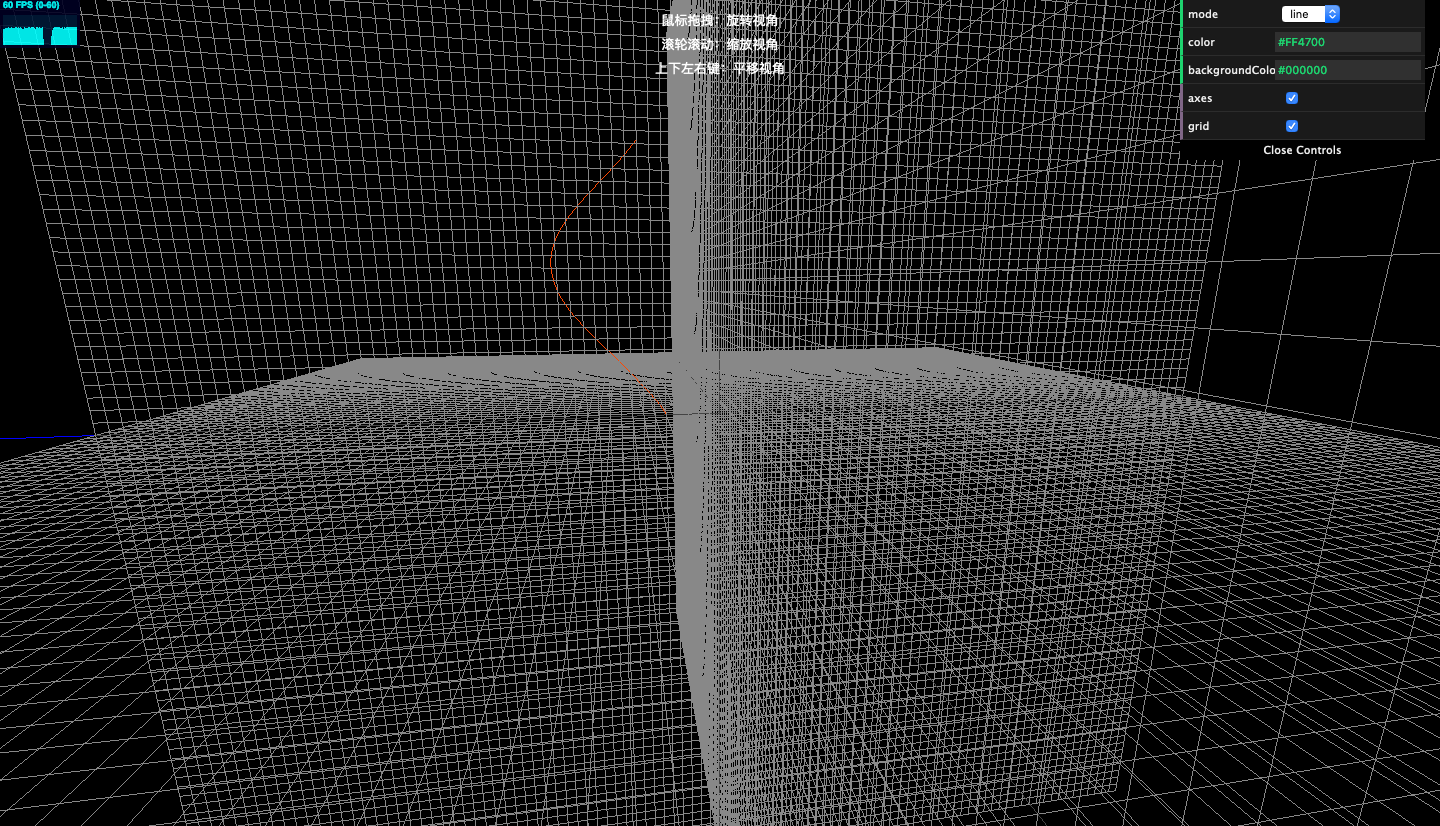
\includegraphics[scale=0.3]{line.png}
\caption{轴线渲染}
\label{fig:line}
\end{figure}

\end{enumerate}

\clearpage

\sectionnonum{总结与展望}

本文基本达到了预期目标,各项功能指标优良。
原始曲率数据入口和WebGL跨平台渲染保证软件的通用性优秀;
HTTPS保证软件的安全性极佳;
在\nameref{sec:error-analyze}中相对误差在$0.03$以内,准确性良好;
实时性虽要考虑网络带宽等不确定因素,但至少在\nameref{sec:pre}中渲染稳定在60帧,表现极佳。

在软件构建技术方面,使用的全部是当代较为先进的技术。
其中WebSocket正支持着成千上万的应用;
TLS保障着整个互联网的安全;
Rust正在为Firefox添砖加瓦;
WebGL定义了下一代的三维渲染应用;
TypeScript是JavaScript社区最受欢迎的转译语言。

在软件架构方面,渲染任务分离。
服务器负责重建,所有的客户端 (浏览器)共享同一份重建数据并渲染。它
大大减少了重建算法的计算压力,仅需一个强有力的服务器完成一次重建,所有的客户端都可以共享重建结果。 
同时,它大大提升了用户的使用体验。在这种架构下,传感器、服务器和客户端即使放置在地球上有互联网覆盖的任意三点,
服务也不会中断。并且终端用户也无需从特定的机器或软件访问服务,而只需要打开任何支持WebGL和TLS
技术的浏览器,即可安全快捷地获得服务。

但在完成度方面,该软件只达到了最小可用的要求,它还需要根据实际需求添加更多的功能以及对现有功能进行调整。
比如添加用户认证系统或者动态分析渲染结果。

要构建一个成熟的三维可视化软件,还有许多工作要做,许多问题有待解决。
